\subsection{Discos rígidos}
\label{subsection:Discos}
Os discos rígidos mais popularmente conhecidos como HD (Hard Disk) é o método mais utilizado para armazenamento de dados pelo computador. utilizando-se de braços metálicos posicionados acima de um disco metálico este gera um pulso eletro magnético para gravar a informação no prato metálico em formato de disco. Tecnologia de desenvolvida em 1956 contava apenas com 5 megabytes de tamanho de armazenamento hoje existem discos com capacidade de armazenamento maior que 10 terabytes \cite{Tanenbaum2016}, \cite{Comer2012}.\\
Normalmente o sistema operacional é gravado  neste disco por ele não ser volátil, ou seja não se apaga mesmo quando o computador está desligado \cite{Tanenbaum2016}, \cite{Comer2012}.\\

\begin{figure}[htpb]
    \centering
   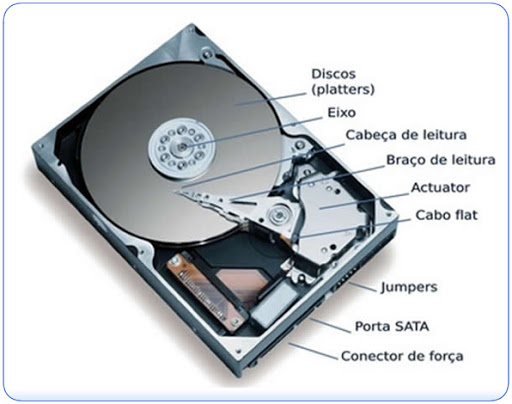
\includegraphics[scale=0.25]{imagens/disco.jpg}
   \caption{Visão de um disco rigido.}
   \label{fig:disco}
\end{figure}